\section{Quantità di vegetazione in alveo}
Si è quantificato l'areale delle isole presenti in alveo avendo accortezza di distinguerlo chiaramente dall'areale della \emph{floodplain}, il quale è soggetto a dinamiche diverse rispetto alle isole.

\subsection{Metodi: classificare l'alveo}
Per classificare il terreno occupato dall'alveo è stato seguito l'approccio di altri autori in analisi simili eseguite su immagini \AST{} e LandSat~TM \squarecites{Bertoldi:2011-ASTER}{Henshaw:2013-LandSat}.
%
\begin{description}
	\item[Maschera computazionale] 
	Dapprima è stata individuata manualmente una maschera di calcolo che comprendesse l'alveo attivo e la parte di piana alluvionale che è stata erosa quando coinvolta nelle piene; 
	tale maschera si estende da Tolmezzo al ponte di Madrisio
	(\cref{fig:esempio-maschera}). 
	Applicandola, il dominio computazionale è stato ridotto a comprendere l'inviluppo degli alvei attivi che si sono succeduti dall'immagine del~2000 a quella del~2018.
	%
	\begin{figure}[t]
		\centering
		\begin{subfigure}[b]{0.4\textwidth}
			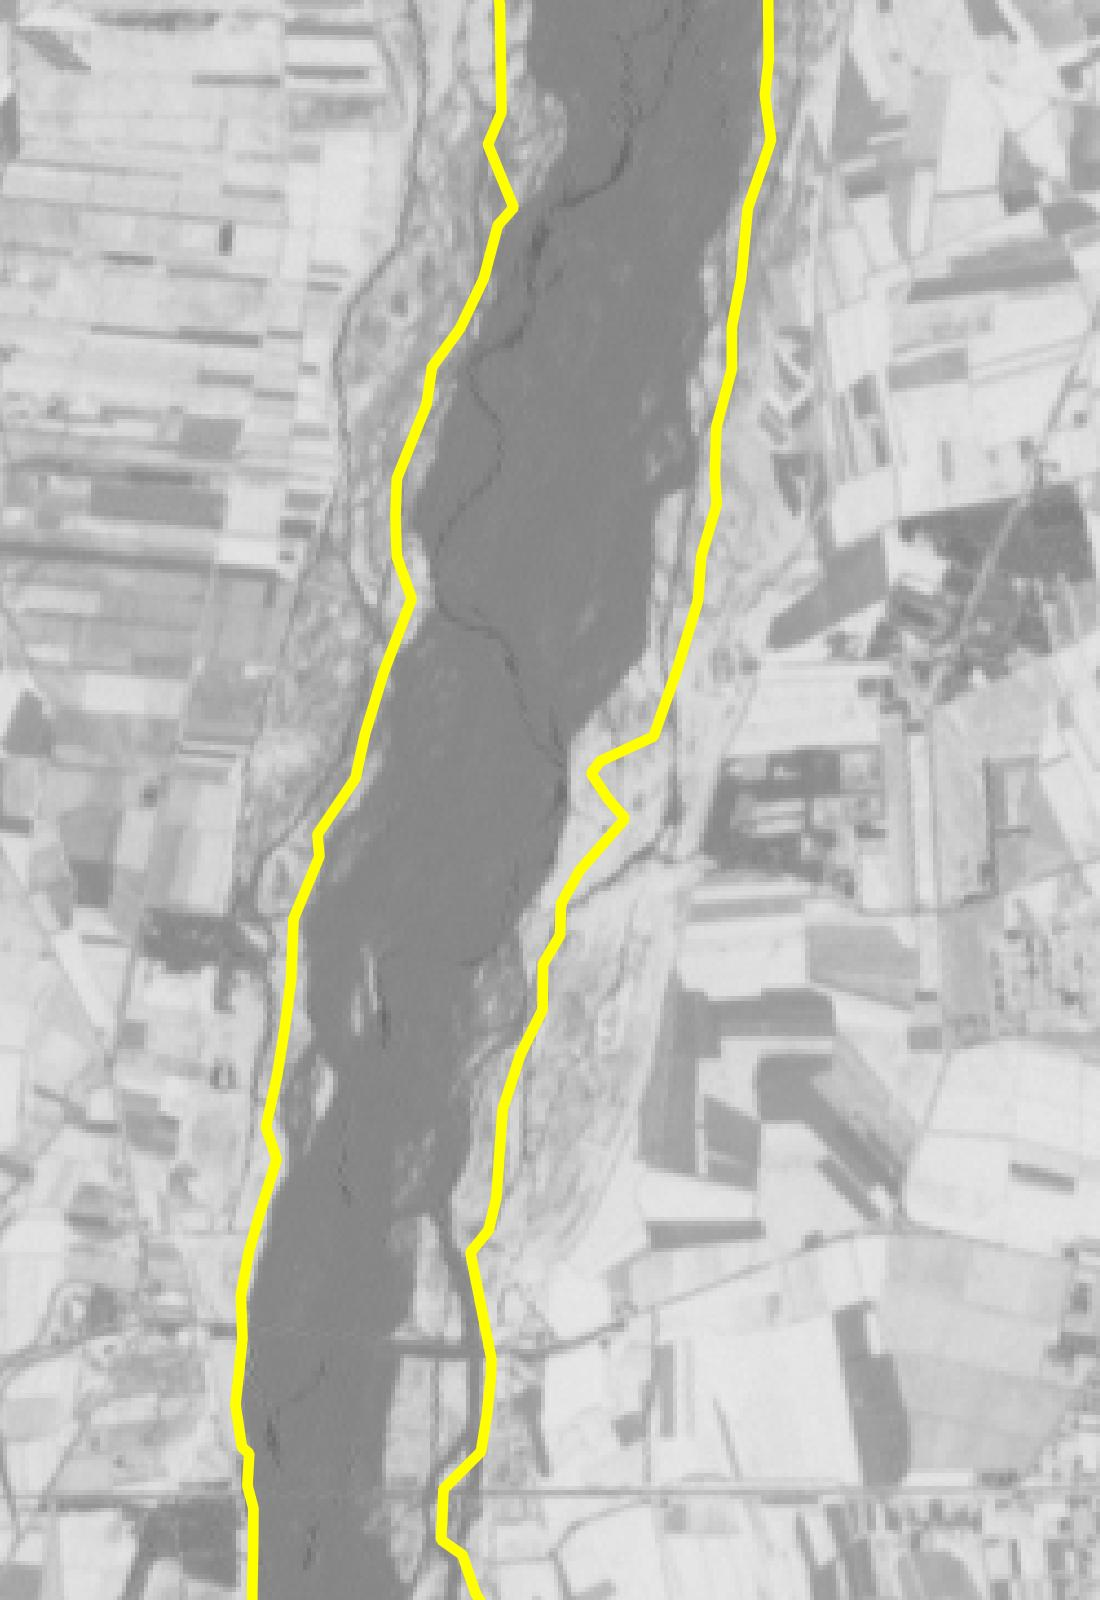
\includegraphics[width=\textwidth]{files/esempio_mask_2002_06_12.jpeg}
			\caption{\AST{} 2002-06-12.}
		\end{subfigure}
		\qquad
		\begin{subfigure}[b]{0.4\textwidth}
			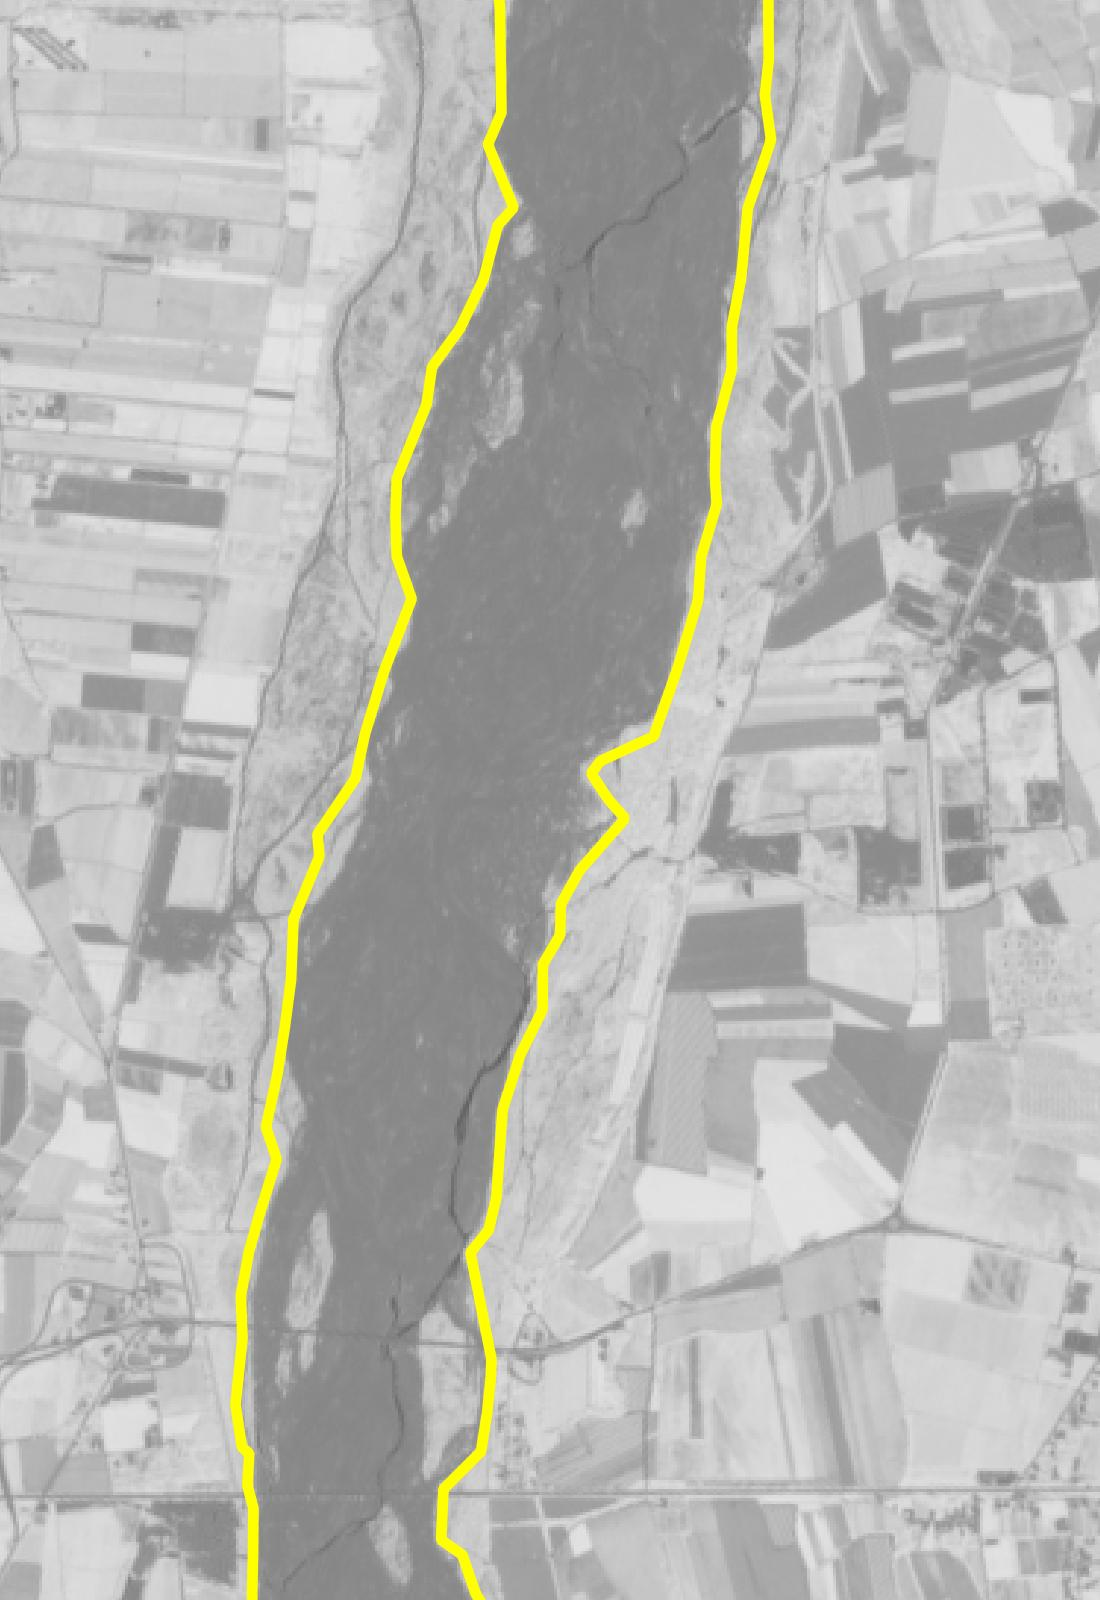
\includegraphics[width=\textwidth]{files/esempio_mask_2015_09_12.jpeg}
			\caption{\Se{} 2015-09-12.}
		\end{subfigure}
		\caption[definizione della maschera per limitare il dominio computazionale]
			{esempio in cui si vede come la maschera utilizzata per limitare il dominio computazionale (in giallo) sia il risultato dell'inviluppo degli alvei attivi che si sono modificati nel tempo; le immagini sono le mappe di NDVI.}
		\label{fig:esempio-maschera}
	\end{figure}
	%
	%
	\item[NDVI] 
	In questa area è stato calcolato il \emph{Normalized Difference Vegetation Index} (NDVI) grazie alle bande del \emph{Near Infrared} (NIR) e del \emph{Red} (R)
	%
	\begin{equation}
		%\notag
		NDVI = \frac{NIR - R}{NIR + R} \quad .
		\label{eq:ndvi}
	\end{equation}
	%
	%
	\item[Aree campione]
	\`{E} stata effettuata una digitalizzazione manuale di alcune aree campione per le immagini \AST{} del~2005-08-30 ($\sim 70$) e del~2012-08-01 ($\sim 100$), le immagini Plaiades del~2014-10-31 ($\sim 40$) e del~2015-06-13 ($\sim 40$), l'immagine \Se{} del~2017-04-21 ($\sim 45$) e l'immagine \WV{} del 2018-06-15 ($\sim 55$) (\cref{fig:esempio-aree-campione}).
	Sono state selezionate immagini per ogni satellite poiché ciascuno è sensibile a bande leggermente diverse. 
	\\
	Queste aree campione sono state suddivise in tre classi: vegetazione, alveo attivo e canale.
	%
	\begin{figure}[ht]
		\centering
		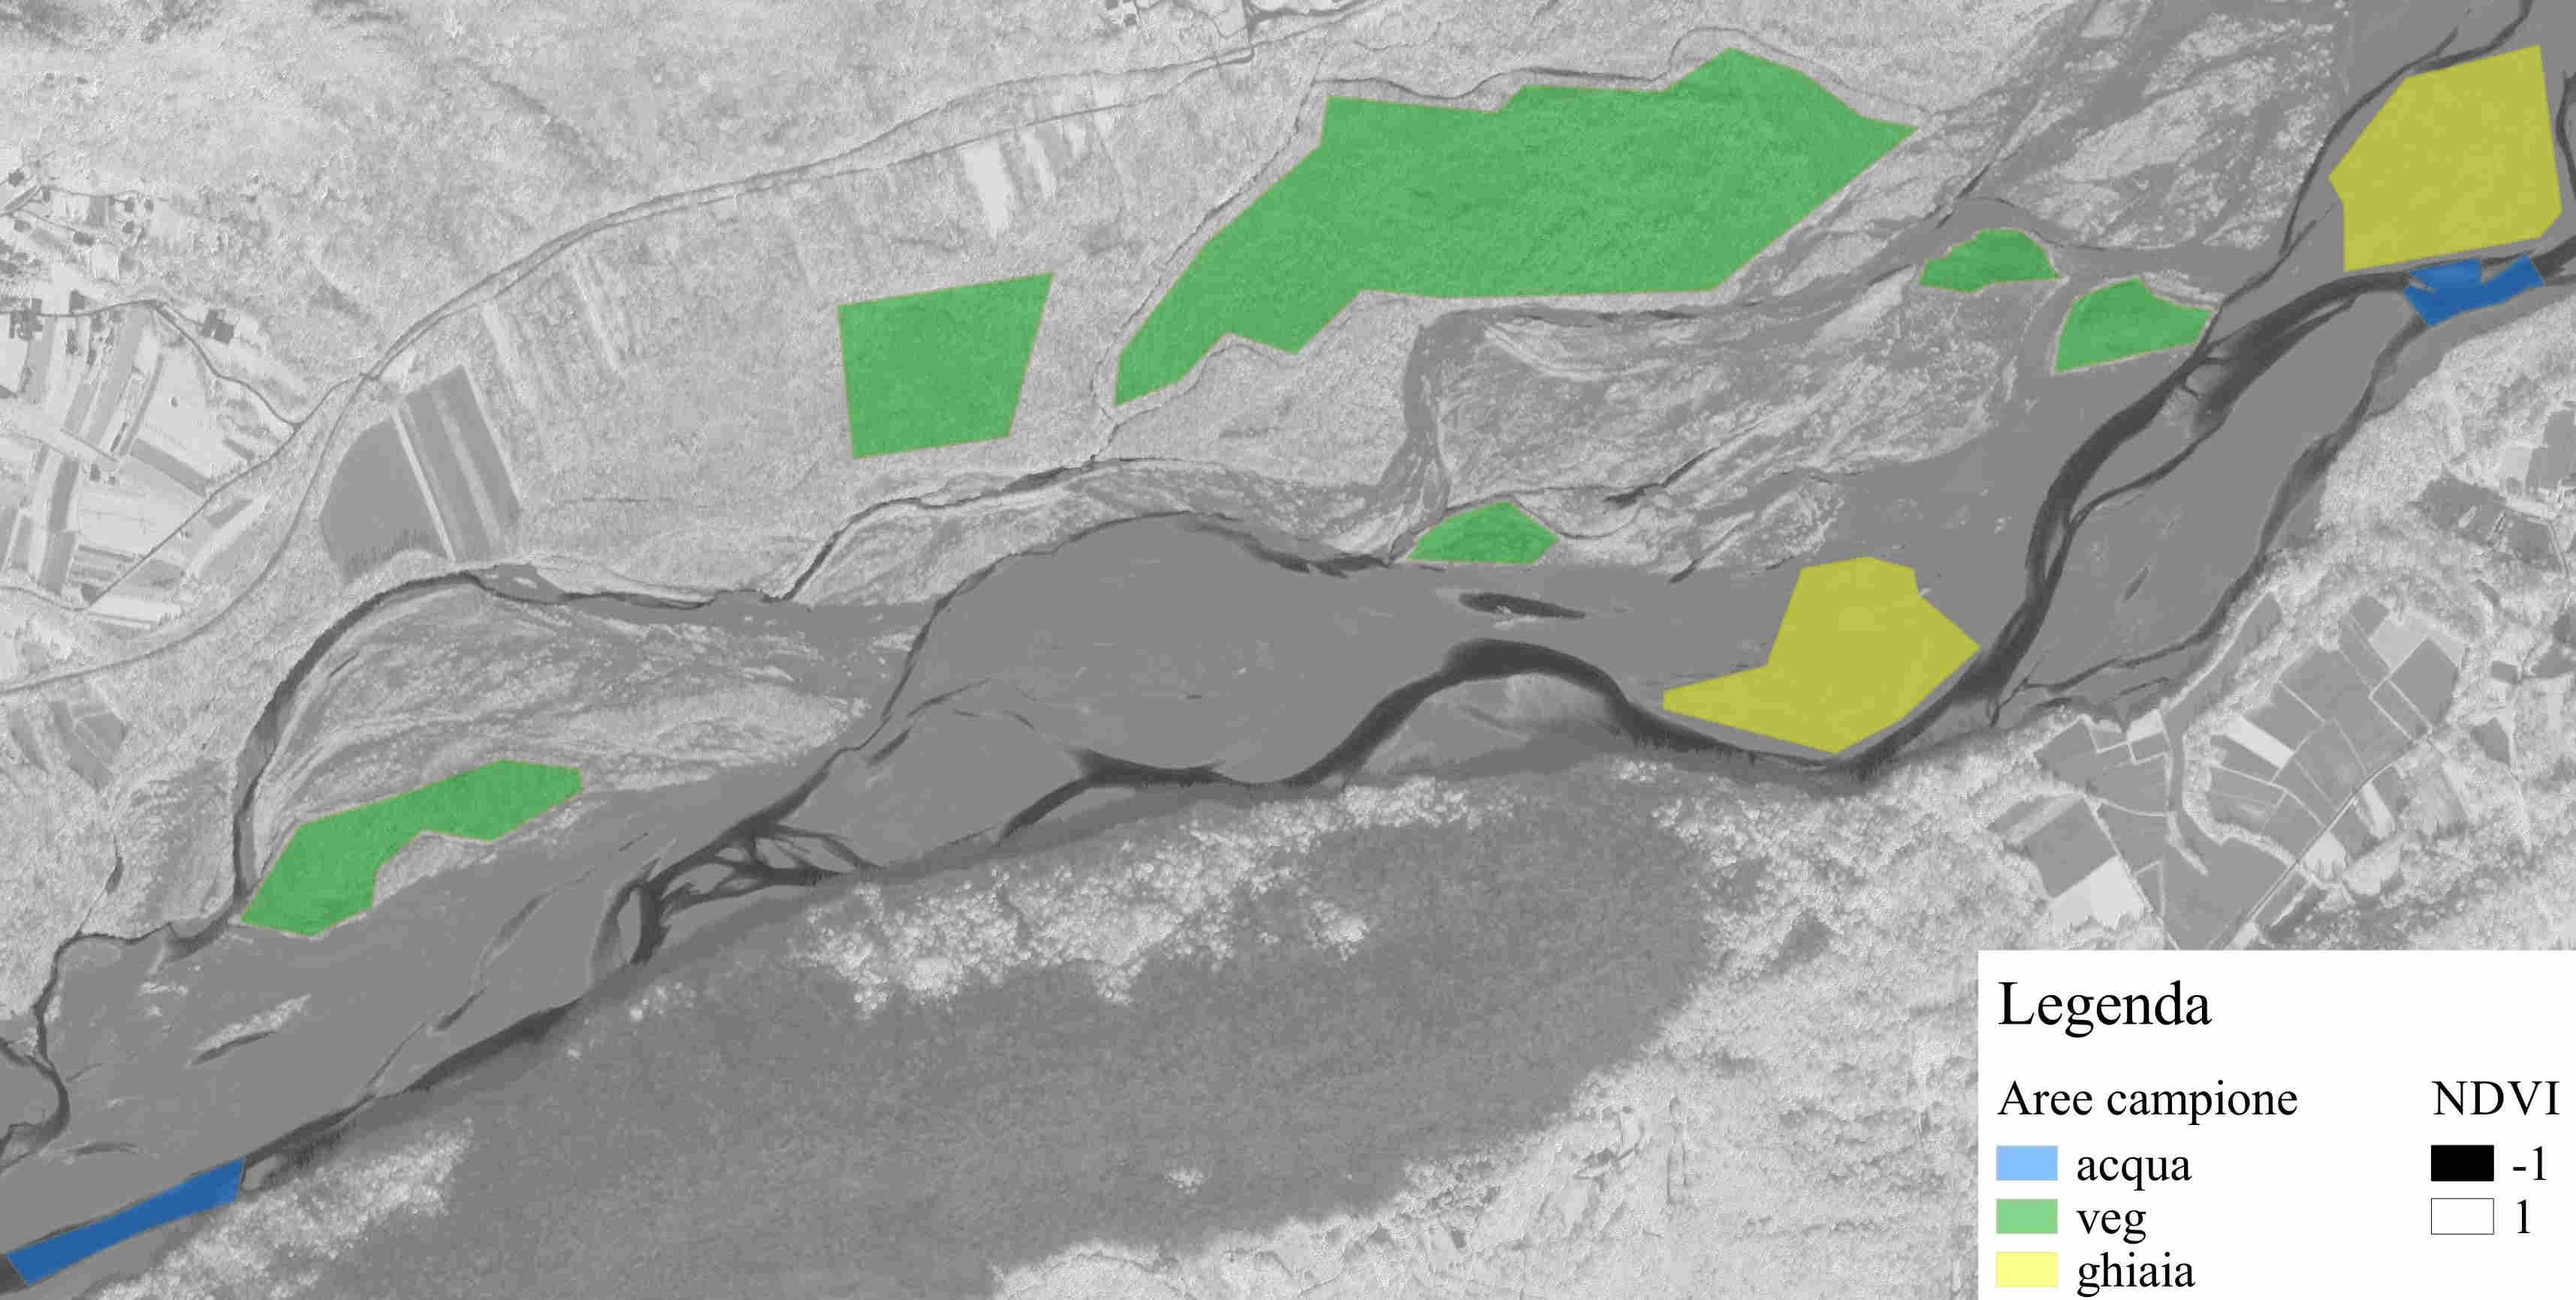
\includegraphics[width=\textwidth]{files/esempio_aree_campione_2014_10_31.jpeg}
		\caption[esempio di aree campione per calcolare la distribuzione dell'NDVI]{esempio di digitalizzazione di alcune aree campione per l'immagine \Pl{} del~2014-10-31; sullo sfondo la mappa dell'NDVI.}
		\label{fig:esempio-aree-campione}
	\end{figure}
	%
	%
	\item[Percentili aree campione]
	Per ogni immagine si è osservata la distribuzione dell'NDVI in ogni classe (\cref{graph:percentili}).
	% 
	\begin{figure}[ht]
		\centering
		\begin{tikzpicture}
	\begin{groupplot}[
		group style = {
			group size = 2 by 3,
			ylabels at = edge left,
			x descriptions at = edge bottom,
			horizontal sep = 1.1cm,
			vertical sep = 0.1cm,
		},
		width = 0.45\textwidth,
		height = 0.45\textwidth,
		ylabel = NDVI,
		boxplot/draw direction = y,
		xtick = {1,2,3},
		xticklabels = {Veg., Alveo, Canale},
		ymax = 0.795,
		ymin = -0.50,
		grid = major,
	]
	\nextgroupplot % ASTER 2005-08-31
		\addplot+ [ % vegetazione
			teal, very thick,
			boxplot prepared = {
				lower whisker = 0.353656,
				lower quartile = 0.470411,
				median = 0.560063,
				upper quartile = 0.614701,
				upper whisker = 0.644957,
				},
        	]
        	coordinates {};
		\addplot+ [ % alveo attivo
			brown, very thick,
			boxplot prepared = {
				lower whisker = 0.077472,
				lower quartile = 0.091653,
				median = 0.122488,
				upper quartile = 0.149573,
				upper whisker = 0.171459,
				},
        	]
        	coordinates {};
		\addplot+ [ % canale
			cyan, very thick,
			boxplot prepared = {
				lower whisker = -0.477885,
				lower quartile = -0.362798,
				median = -0.269905,
				upper quartile = -0.058787,
				upper whisker = 0.072414,
				},
        	]
        	coordinates {};
        \node [fill = white, draw = black, anchor = north east] 
        	at (axis description cs: 1,1) {AST 2005-08-31};
	%------------------------------------------------------
	\nextgroupplot % ASTER 2012-08-01
		\addplot+ [ % vegetazione
			teal, very thick,
			boxplot prepared = {
				lower whisker = 0.341613,
				lower quartile = 0.444200,
				median = 0.586294,
				upper quartile = 0.672889,
				upper whisker = 0.709027,
				},
        	]
        	coordinates {};
		\addplot+ [ % alveo attivo
			brown, very thick,
			boxplot prepared = {
				lower whisker = 0.10506,
				lower quartile = 0.117969,
				median = 0.143631,
				upper quartile = 0.16549,
				upper whisker = 0.184871,
				},
        	]
        	coordinates {};
		\addplot+ [ % canale
			cyan, very thick,
			boxplot prepared = {
				lower whisker = -0.432201,
				lower quartile = -0.379825,
				median = -0.322239,
				upper quartile = -0.226459,
				upper whisker = -0.103914,
				},
        	]
        	coordinates {};
        \node [fill = white, draw = black, anchor = north east] 
        	at (axis description cs: 1,1) {AST 2012-08-01};
	%------------------------------------------------------
	\nextgroupplot % Pleiades 2014-10-31
		\addplot+ [ % vegetazione
			teal, very thick,
			boxplot prepared = {
				lower whisker = 0.286467,
				lower quartile = 0.350238,
				median = 0.415502,
				upper quartile = 0.483495,
				upper whisker = 0.549505,
				},
        	]
        	coordinates {};
		\addplot+ [ % alveo attivo
			brown, very thick,
			boxplot prepared = {
				lower whisker = 0.049796,
				lower quartile = 0.055794,
				median = 0.063049,
				upper quartile = 0.07173,
				upper whisker = 0.081427,
				},
        	]
        	coordinates {};
		\addplot+ [ % canale
			cyan, very thick,
			boxplot prepared = {
				lower whisker = -0.426415,
				lower quartile = -0.387978,
				median = -0.338308,
				upper quartile = -0.266515,
				upper whisker = -0.175373,
				},
        	]
        	coordinates {};
        \node [fill = white, draw = black, anchor = north east] 
        	at (axis description cs: 1,1) {PL 2014-10-31};
	%------------------------------------------------------
	\nextgroupplot % Pleiades 2015-08-13
		\addplot+ [ % vegetazione
			teal, very thick,
			boxplot prepared = {
				lower whisker = 0.415693,
				lower quartile = 0.5,
				median = 0.570359,
				upper quartile = 0.638507,
				upper whisker = 0.704044		
,
				},
        	]
        	coordinates {};
		\addplot+ [ % alveo attivo
			brown, very thick,
			boxplot prepared = {
				lower whisker = 0.075052,
				lower quartile = 0.080858,
				median = 0.087921,
				upper quartile = 0.096031,
				upper whisker = 0.106198,
				},
        	]
        	coordinates {};
		\addplot+ [ % canale
			cyan, very thick,
			boxplot prepared = {
				lower whisker = -0.262599,
				lower quartile = -0.244228,
				median = -0.214393,
				upper quartile = -0.176471,
				upper whisker = -0.132762,
				},
        	]
        	coordinates {};
        \node [fill = white, draw = black, anchor = north east] 
        	at (axis description cs: 1,1) {PL 2015-08-13};
	%------------------------------------------------------
	\nextgroupplot % Sentinel2 2017-04-21
		\addplot+ [ % vegetazione
			teal, very thick,
			boxplot prepared = {
				lower whisker = 0.163722,
				lower quartile = 0.241916,
				median = 0.374344,
				upper quartile = 0.548241,
				upper whisker = 0.672782,
				},
        	]
        	coordinates {};
		\addplot+ [ % alveo attivo
			brown, very thick,
			boxplot prepared = {
				lower whisker = 0.056176,
				lower quartile = 0.061278,
				median = 0.067681,
				upper quartile = 0.076396,
				upper whisker = 0.089304,
				},
        	]
        	coordinates {};
		\addplot+ [ % canale
			cyan, very thick,
			boxplot prepared = {
				lower whisker = -0.322237,
				lower quartile = -0.288822,
				median = -0.239533,
				upper quartile = -0.177094,
				upper whisker = -0.131119,
				},
        	]
        	coordinates {};
        \node [fill = white, draw = black, anchor = north east] 
        	at (axis description cs: 1,1) {S2 2017-04-21};
	%------------------------------------------------------
	\nextgroupplot % WorldView2 2018-06-15
		\addplot+ [ % vegetazione
			teal, very thick,
			boxplot prepared = {
				lower whisker = 0.569665,
				lower quartile = 0.657917,
				median = 0.719523,
				upper quartile = 0.759148,
				upper whisker = 0.791594,
				},
        	]
        	coordinates {};
		\addplot+ [ % alveo attivo
			brown, very thick,
			boxplot prepared = {
				lower whisker = 0.126214,
				lower quartile = 0.129661,
				median = 0.13373,
				upper quartile = 0.138542,
				upper whisker = 0.149326,
				},
        	]
        	coordinates {};
		\addplot+ [ % canale
			cyan, very thick,
			boxplot prepared = {
				lower whisker = -0.416974,
				lower quartile = -0.392405,
				median = -0.365385,
				upper quartile = -0.335135,
				upper whisker = -0.29979,
				},
        	]
        	coordinates {};
        \node [fill = white, draw = black, anchor = north east] 
        	at (axis description cs: 1,1) {WV2 2018-06-15};
	\end{groupplot}
\end{tikzpicture}

		\caption[\emph{boxplot} dell'NDVI nelle aree campione in quattro immagini satellitari]{\emph{boxplot} dell'NDVI nelle aree campione in quattro immagini satellitari; i baffi indicano il 10mo e il 90mo percentile, gli estremi della scatola rappresentano il 25mo e il 75mo percentile, la linea nella scatola è la mediana.}
		\label{graph:percentili}
	\end{figure}
	%
	%
	\item[Soglie NDVI] 
	Da tali grafici sono state ottenute delle soglie di NDVI per classificare le immagini satellitari (\cref{tab:ndvi-soglia}); per l'immagine \WV{} la soglia che distingue vegetazione da alveo attivo è maggiore. 
	Le soglie sono leggermente maggiori a quanto riportato in letteratura \squarecites{Bertoldi:2011-ASTER}{Henshaw:2013-LandSat} poiché in questo modo c'è una maggior corrispondenza con i dati utilizzati per validare il processo (riportati di seguito).
	%
	\begin{table}[ht]
		\centering
		\begin{tabular}{
			c 
			S[table-format=1.2]@{\,}
			c@{\,}
			c@{\,}
			c@{\,}
			S[table-format=1.2]
			S[table-format=1.1]@{\,}
			c@{\,}
			c@{\,}
			c@{\,}
			S[table-format=1.1]
			}
			\toprule
			&	\multicolumn{5}{c}{\textbf{Soglie AST PL S2}}	&	\multicolumn{5}{c}{\textbf{Soglie WV2}}	\\
			\midrule
			Vegetazione		&	0.25	&	$\leq$	&	NDVI	&			&		& 	0.3	&	$\leq$	&	NDVI	&			& 	\\
			Alveo attivo	&	0.0	&	$\leq$	&	NDVI	&	$<$		&	0.25	&	0.0	&	$\leq$	&	NDVI	&	$<$		&	0.3\\
			Canale			&		&			&	NDVI	&	$<$		&	0.0	&		&			&	NDVI	&	$<$		&	0.0\\
			\bottomrule
		\end{tabular}
		\caption[soglie NDVI]{soglie di NDVI per la classificazione delle immagini satellitari.}
		\label{tab:ndvi-soglia}
	\end{table}
	%
	%
	\item[Isole e \emph{Floodplain}]
	Tramite una procedura semi-automatica e con il supporto di Google Earth, la classe della vegetazione è stata suddivisa in \emph{floodplain} e isole. 
	Tale procedura si basa sul fatto che la maschera computazionale comprende parte della piana alluvionale e che le isole sono completamente circondate dalla ghiaia dell'alveo durante periodi di magra.
	\\
	Successivamente, un controllo visivo del risultato e una correzione manuale di alcune celle hanno permesso sia di distinguere correttamente le isole, sia di evitare che isole molto prossime alla \emph{floodplain} ne fossero considerate parte; la classe delle celle corrette è stata aggiunta alla classificazione.
	%
	%
	\item[Nuvole e nodata] Alcune immagini presentano una lieve copertura nuvolosa che si estende nella maschera; queste zone sono state manualmente delimitate poiché presentano valori NDVI alterati.
	\\
	Altre immagini hanno un'estensione limitata rispetto alla maschera; questo porta ad avere aree prive di dati (\texttt{nodata}).
	\\
	Alla classificazione sono state aggiunte la classe delle nuvole e dei \texttt{nodata}.
	%
	%
	\item[Classificazione finale dei tratti] La \cref{tab:class_tratti} mostra le classi in cui è stato classificato ognuno dei 23~tratti; la \cref{fig:class_is_fl} ne mostra un esempio.
	%
	\begin{table}[ht]
		\centering
		\begin{tabular}{
			c 
			c
			}
			\toprule
			\textbf{Macroclasse}	&	\textbf{Classe}	\\
			\midrule
			Vegetazione		&	Isola	\\
							&	Floodplain	\\
			Alveo attivo	&	Cella corretta	\\
							&	Ghiaia	\\
							&	Canale	\\
			Altro			&	Nuvola	\\
							&	Nodata	\\
			\bottomrule
		\end{tabular}
		\caption[classificazione dell'area dei tratti]{classificazione finale dell'area di ogni tratto all'interno della maschera computazionale.}
		\label{tab:class_tratti}
	\end{table}
	%
	\begin{figure}[ht]
		\centering
		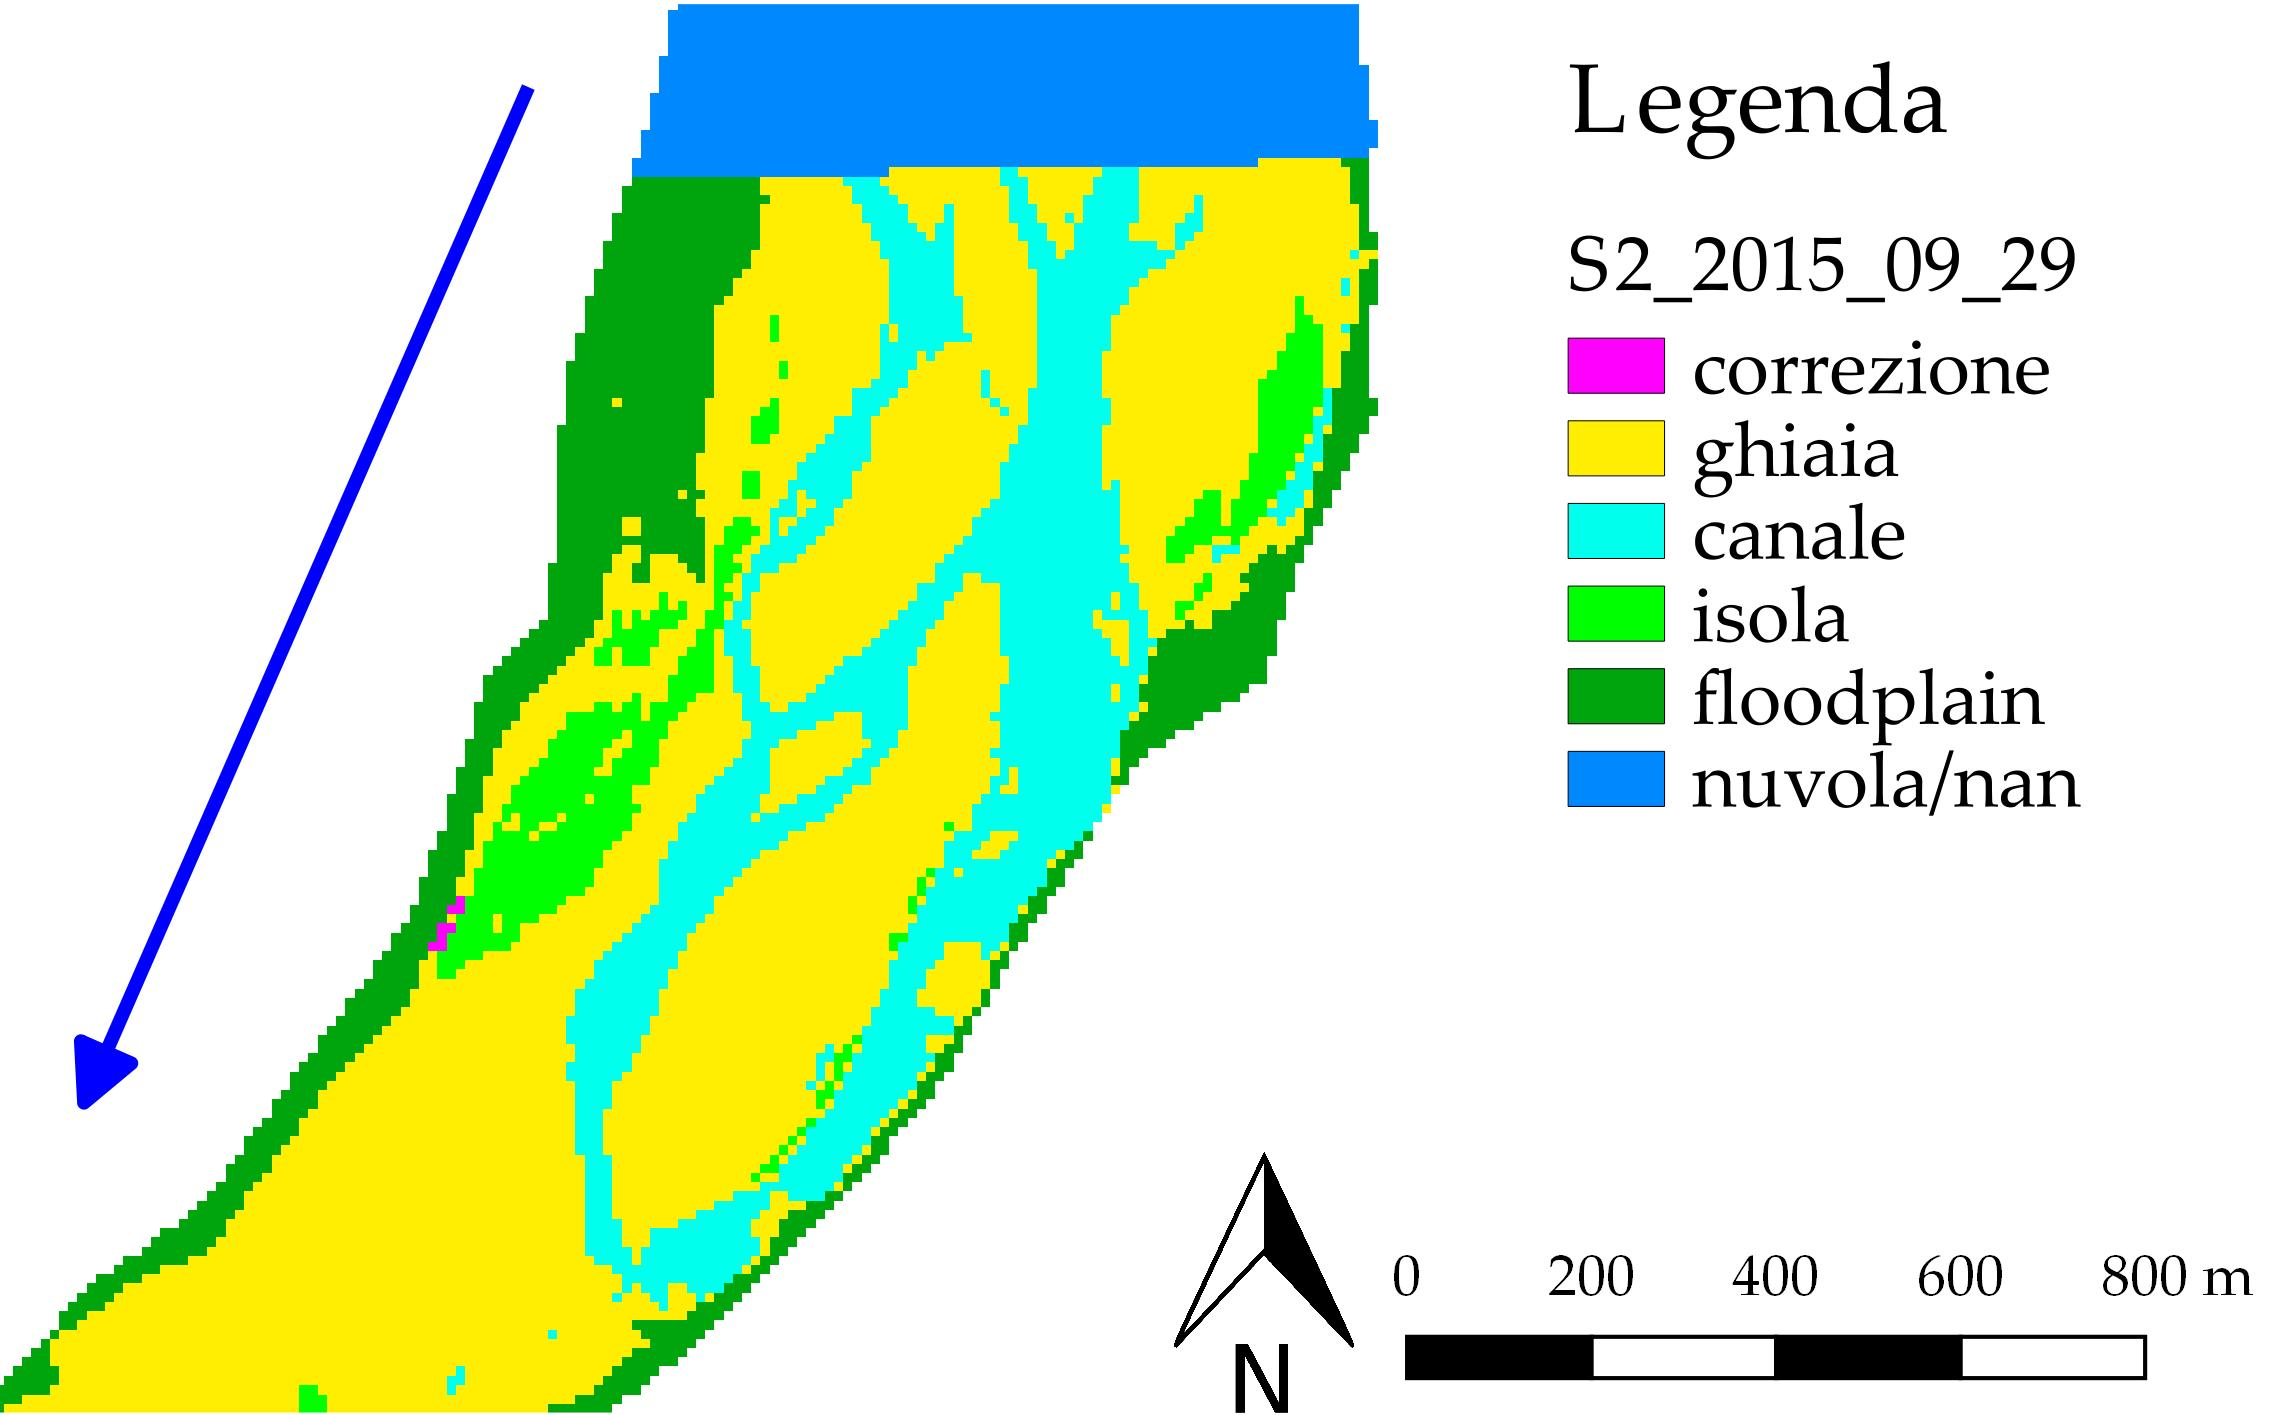
\includegraphics[width=\textwidth]{files/esempio_class_is_fl.jpeg}
		\caption[esempio della classificazione dell'area dei tratti]{esempio della classificazione dell'area dei tratti; le zone raffigurate sono rispettivamente a monte dell'isola di Cornino (in corrispondenza del monte Prat) e in corrispondenza della confluenza del Fella.}
		\label{fig:class_is_fl}
	\end{figure}
	%
Al fine di validare la precedente procedura di controllo e correzione della distinzione isole - \emph{floodplain}, si è osservato per ogni tratto l'andamento temporale della larghezza media~$B$, esprimibile semplicemente come il rapporto dell'area dell'alveo di ogni tratto (somma dell'alveo attivo e delle isole) per la sua lunghezza seguendo la corrente:
	%
	\begin{equation}
		\label{eq:larghezza-tratto}
		B = \frac{\text{Area alveo}}{Lunghezza} 
		\quad 
		\si{[\m]}
		\quad.
	\end{equation}
	% 
	Si è verificato che la larghezza~$B$ rimanesse costante nel tempo, indice di una corretta classificazione tra isole e \emph{floodplain}. 
	La~$B$ non rimane costante solo nel caso di distacco di isole o di fusione di isole nella piana. 
	\\
	La \cref{fig:b-media-7-e-15} mostra l'andamento temporale della~$B$ dei tratti~7 e~15: nel primo tratto, in cui non si osserva alcuna variazione sensibile dell'alveo, la~$B$ oscilla solo di qualche decina di metri; nel secondo si assiste alla progressiva fusione di una grande isola nella \emph{floodplain}, e questo lo si vede proprio nella diminuzione della~$B$. Ciò che conta non è quanto è largo l'alveo, ma quanto cambia la larghezza.
	%
	\begin{figure}
		\centering
		\begin{tikzpicture}
	\begin{axis}[
		width = 0.6\textwidth,
		height = 0.5\textwidth,
		date coordinates in = x,
		xticklabel = {\year},
		xticklabel style = {
			rotate = 80,
			anchor = near xticklabel
		},
		xtick distance = 730,
		enlarge x limits = 0.05,
		enlarge y limits = 0.01,
		%ymax = 3.7,
		%ymin = -0.1,
		%ytick distance = 0.5,
		ylabel = {Larghezza media dell'alveo \si{[\m]}},
		grid = major,
		]
		\addplot+
        	[blue]
        	table [x=data, y=tr_7] {graphics/data/Larghezze_medie_alveo.txt};
        \addlegendentry{Tratto 7}
        
		\addplot+
        	[orange]
        	table [x=data, y=tr_15] {graphics/data/Larghezze_medie_alveo.txt};
        \addlegendentry{Tratto 15}
	\end{axis}
\end{tikzpicture}

		\quad
		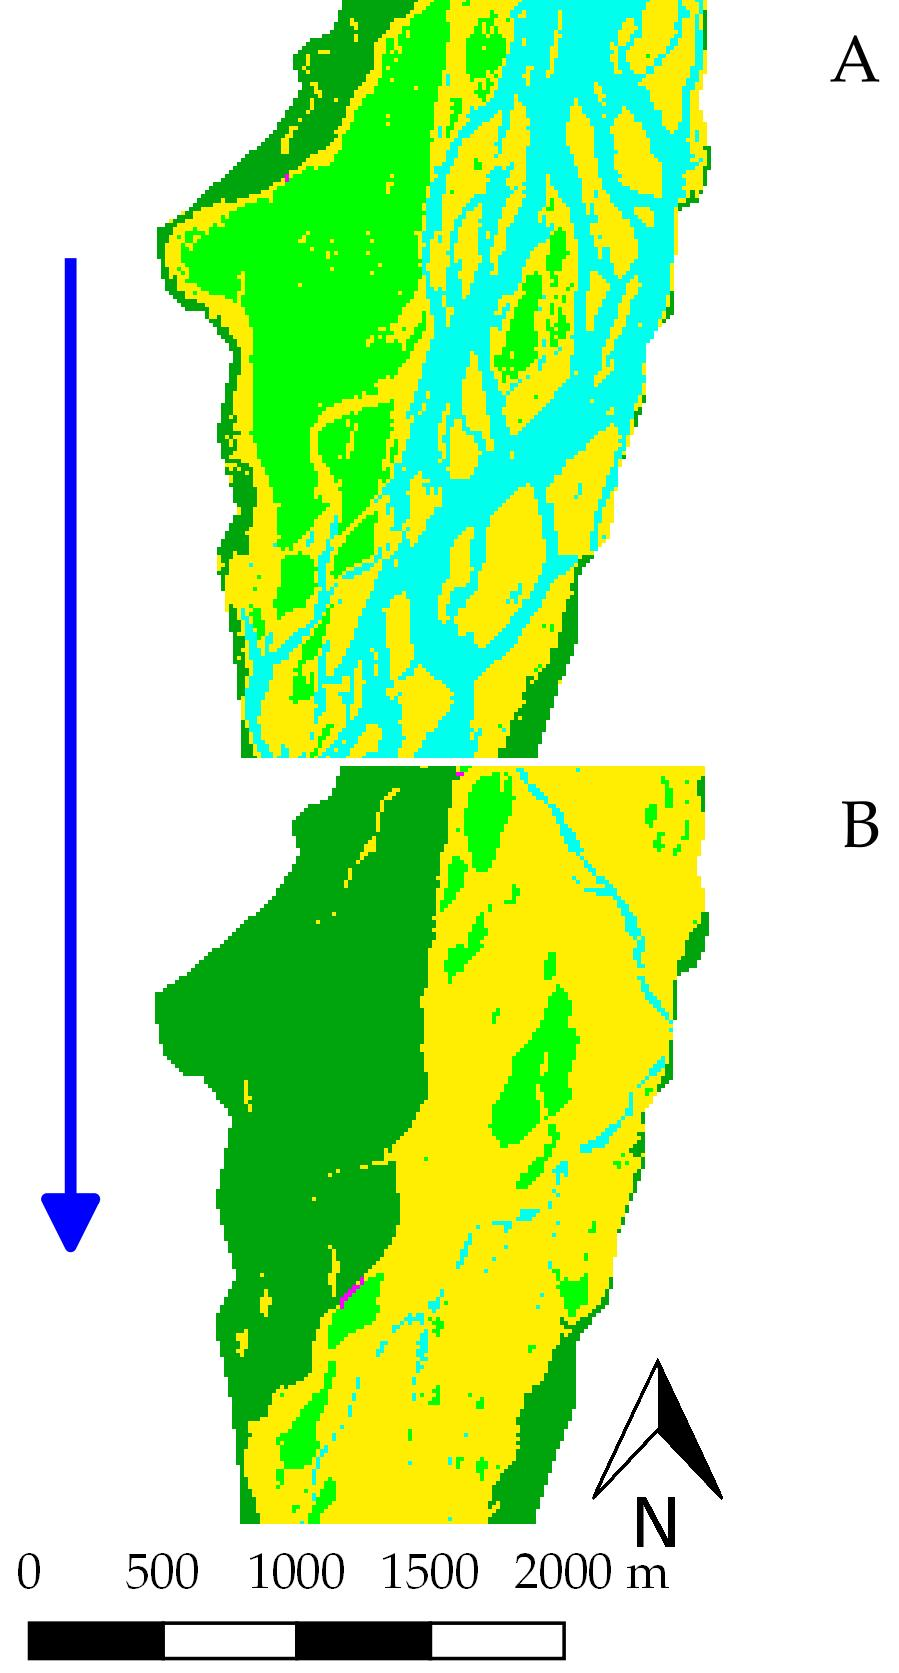
\includegraphics[width=0.3\textwidth]{files/fusione_isola_tr_15.jpeg}
		\caption[andamento temporale di $B$ per i tratti~7 e~15]{a sinistra si vede l'andamento nel tempo della larghezza media dei tratti~7 e~15; la $B$ del tratto~7 oscilla solamente di qualche decina di metri, mentre il tratto~15 riduce improvvisamente la sua $B$ a causa della fusione di una grande isola nella \emph{floodplain}, fenomeno mostrato a destra (A: 2002-06-12, B: 2005-08-30).}
		\label{fig:b-media-7-e-15}
	\end{figure}
	%
	%
	\item[Ulteriore validazione] Si è confrontata la classificazione del 2011-10-02 con la classificazione eseguita manualmente da \squarecite{Surian:2015} nei tratti \numrange[range-phrase={$\div$}]{6}{12} (dal ponte autostradale di Braulins alla stretta di Pinzano).
	Le mappe di classificazione del 2005-08-30, 2010-09-29, 2013-09-05 sono state confrontate con i CHM ricavati dai rilievi aerei LiDAR eseguiti nei corrispondenti anni sui tratti \numrange[range-phrase={$\div$}]{6}{12} (\cref{fig:validazione-class-is-fl}).
	Tra i rilievi LiDAR e le immagini \AST{} non hanno avuto luogo particolari eventi di piena.
	%	
	\begin{figure}
		\centering
		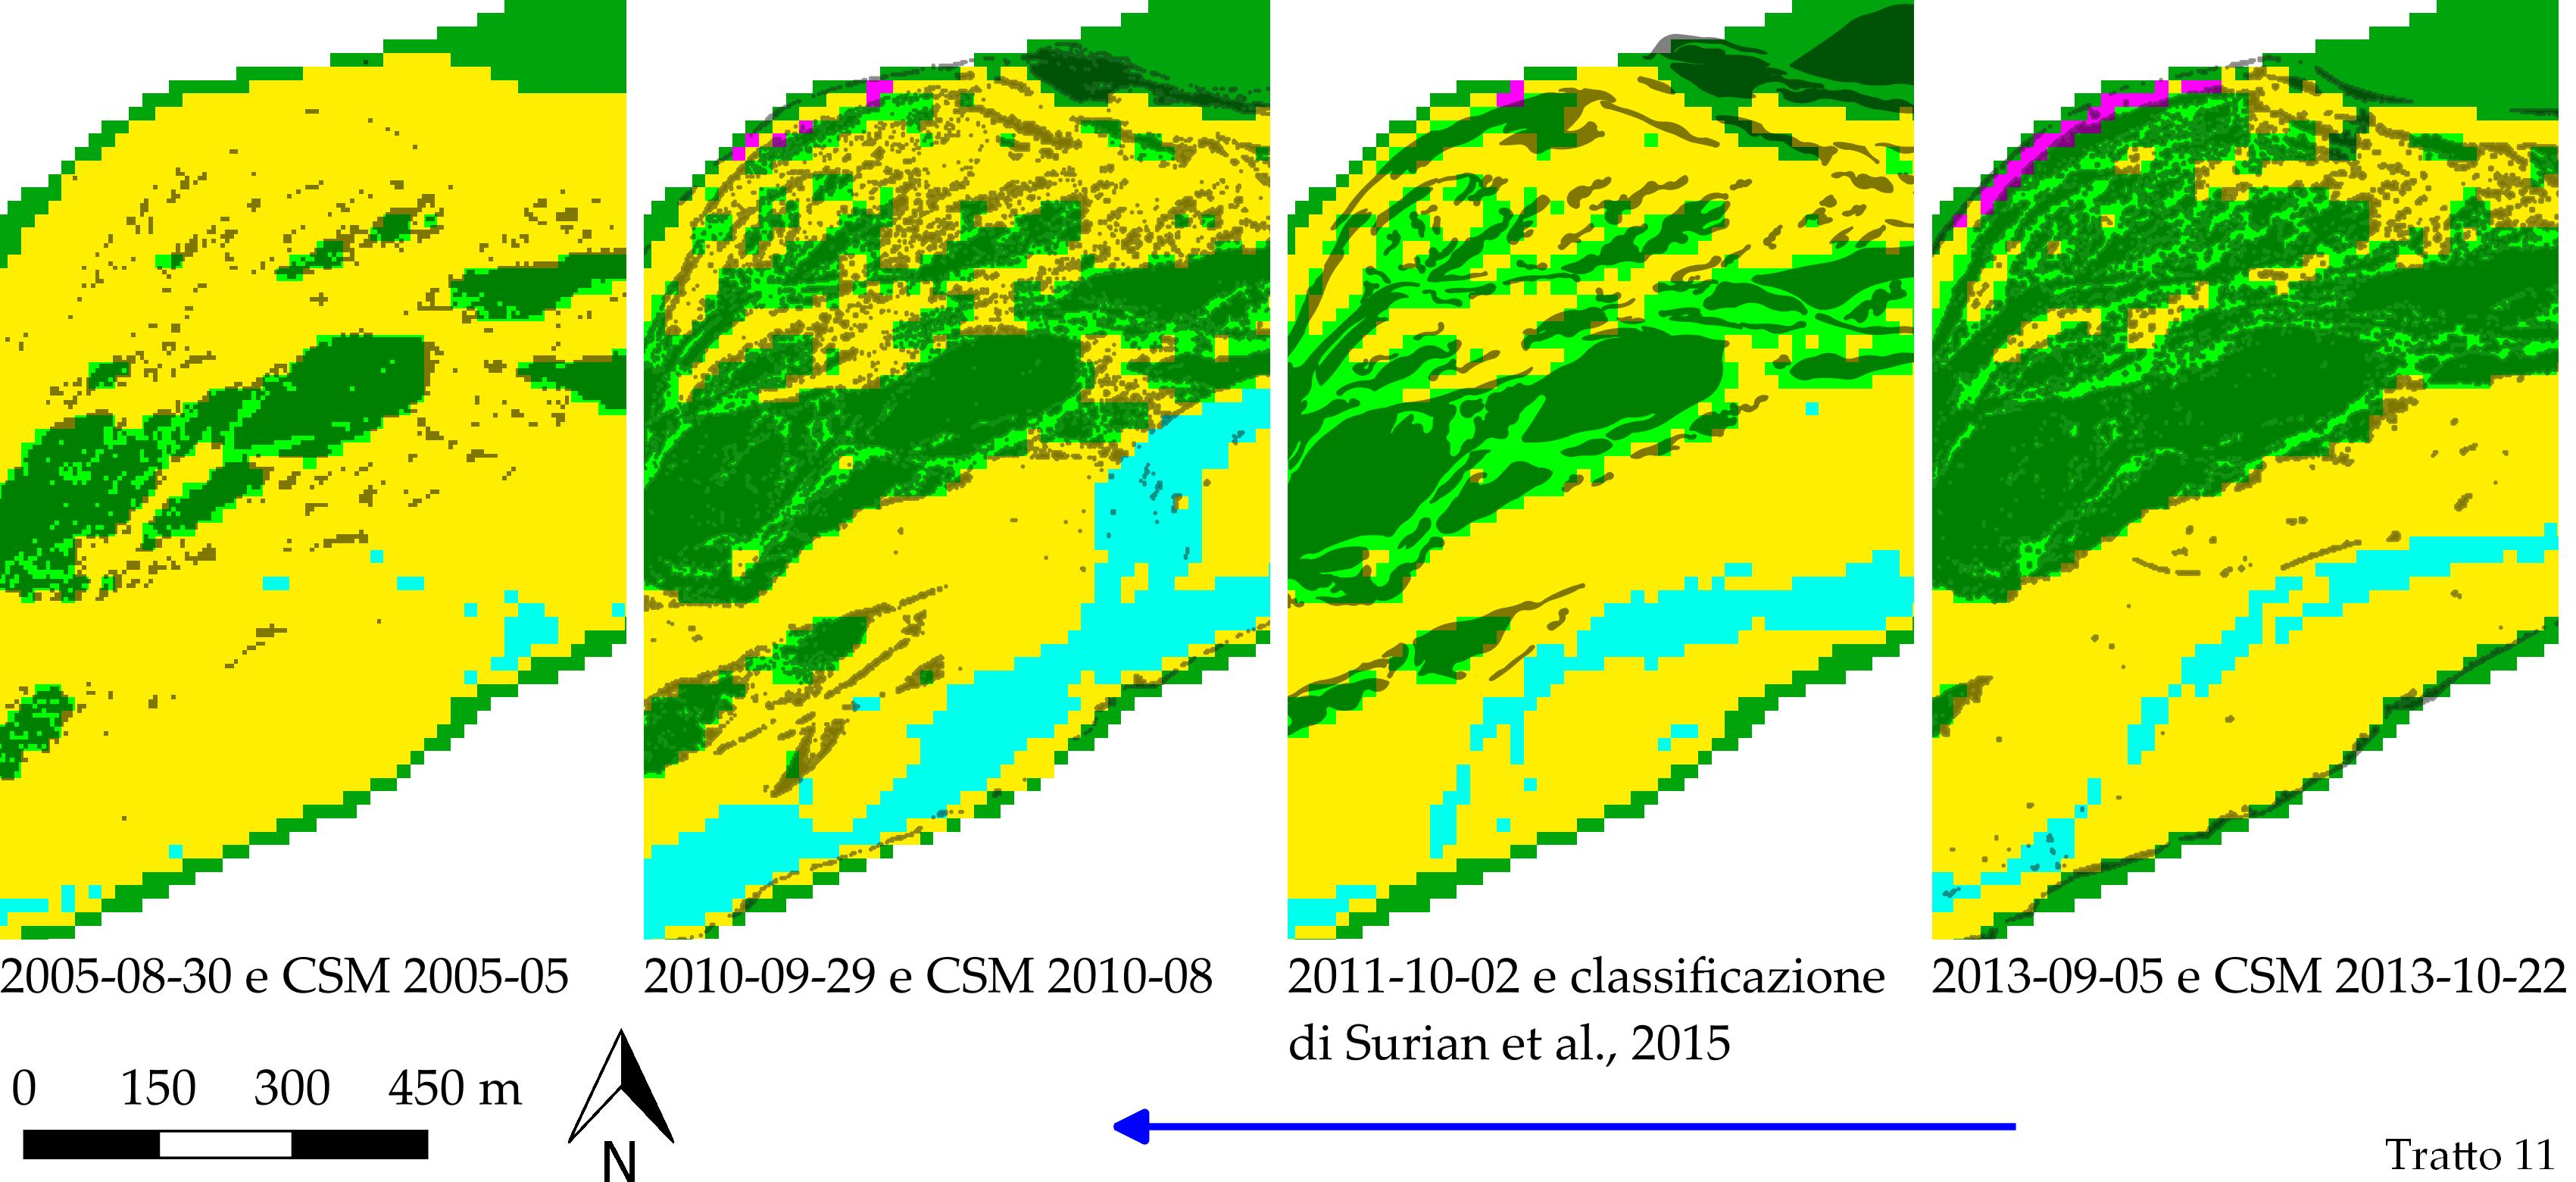
\includegraphics[width=\textwidth]{files/class_mia_vs_surian_chm.jpeg}
		\caption[validazione della classificazione dell'alveo]{confronto tra le mappe di classificazione dell'alveo e i CHM dai rilievi aerei LiDAR e la classificazione manuale eseguita in \squarecite{Surian:2015}; le aree scure corrispondono alla vegetazione individuata nei CHM e dalla classificazione manuale; per la legenda delle mappe di classificazione dell'alveo vedere la \cref{fig:class_is_fl}.}
		\label{fig:validazione-class-is-fl}
	\end{figure}
	%
	\\
	Visualmente si verifiche che c'è sostanziale corrispondenza tra le classificazioni ottenute dalle immagini satellitari e la vegetazione individuata dai CHM, così come tra la classificazione manuale di \squarecite{Surian:2015} e la mappa del 2011-10-22.
	\\
	Esiste una certa differenza tra la classificazione manuale e quella semi-automatica utilizzata nel presente lavoro: la metodologia con cui si procede influisce sul risultato finale.
	Avendo \squarecite{Surian:2015} utilizzato ortofoto ad alta risoluzione (\SI{0.1}{\m}), hanno potuto facilmente distinguere le chiome dei singoli alberi dalla ghiaia o vegetazione bassa circostante; le immagini satellitari utilizzate (principalmente a risoluzione di \SI{10}{\m} o \SI{15}{\m}) permettono invece di osservare macchie di vegetazione.
	In quanto si considera come isola non solo la vegetazione presente all'interno dell'alveo attivo, ma anche la zona meno vegetata posta circa alla medesima quota, l'approccio seguito sembra delineare più nettamente il contorno delle isole maggiori, sebbene le isole più piccole (con estensione minore di una cella) non siano individuate.
	\\
	Un rapido confronto delle mappe di classificazione \Pl{} e \WV{} ad alta risoluzione (\SI{0.5}{\m}) con le mappe di classificazione manuale e il CHM del 2013-10-22 mostra una sovrapposizione quasi completa della vegetazione individuata con i diversi metodi.
	\\
	A fronte di quanto esposto, si ritiene che la classificazione eseguita sia sufficientemente validata.
\end{description}



\FloatBarrier
\subsection{Risultati: evoluzione della larghezza}
Utilizzando le mappe di classificazione del terreno, si è ottenuta una larghezza media~$B$ secondo l'equazione~\eqref{eq:larghezza-tratto}. Questa viene riportata nel grafico in \cref{graph:larghezze-tutti-tratti}, dove si vede la larghezza di ogni tratto valido per ogni immagine disponibile.
%
\begin{figure}
	\centering
	\tikzsetnextfilename{larghezze_tutti_tratti}
\begin{tikzpicture}
	\begin{axis}[
		width = .8\textwidth,
		height = \textwidth,
%		date coordinates in = y,
%		date ZERO = 2000-08-01,
%		yticklabel = {$\year-\month-\day$},
		yticklabel style = {
			rotate = 0,
			anchor = near yticklabel,
		},
		symbolic y coords = {2000-09-17, 2001-06-07, 2002-05-18, 2002-06-12, 2003-06-22, 2004-10-14, 2005-08-30, 2006-07-16, 2007-09-21, 2008-07-05, 2009-07-08, 2010-09-29, 2011-10-02, 2012-08-01, 2013-09-05, 2014-09-08, 2014-10-31, 2015-08-13, 2015-09-12, 2015-10-22, 2016-09-13, 2017-04-21, 2017-06-13, 2018-06-15, 2018-09-16},
		ytick distance = 1.5,
		xticklabel style = {font=\footnotesize},
		xtick = data,
		enlargelimits = 0,
		xlabel = {Tratto},
		colorbar right,
		]
		\addplot[
			matrix plot*,
			mesh/cols = 23,	% per fargli leggere colonne formate da 23 righe dal file di testo
			shader = flat corner,	% per interpolare i colori
		]
        	table [x = tratto, y = data, point meta = \thisrow{larghezza}] {graphics/data/Larghezze_tutti_tratti.txt};
	\end{axis}
\end{tikzpicture}

	\caption[larghezza di tutti i tratti per ogni immagine]{larghezza di tutti i tratti per ogni immagine; i quadrati bianchi indicano assenza di dati (a causa della presenza di nuvole o limitata estensione dell'immagine).}
	\label{graph:larghezze-tutti-tratti}
\end{figure}
%
\\
Ogni “fetta” verticale del grafico corrisponde ad un'istantanea temporale: in quella specifica data, i tratti del Tagliamento avevano quella specifica larghezza.
Già così si vede quanto era stato descritto nell'introduzione:
i primi tratti sono quelli più stretti poiché confinati dalle montagne;
si osserva un progressivo allargamento all'incirca dal ponte autostradale di Braulins (a monte del tratto~6), interrotto dalla stretta di Pinzano (a valle del tratto~12);
infine, al successivo riallargamento dei tratti planiziali segue il cambio morfologico e il corrispondente restringimento (dal tratto~22).
Questo trend è costante nel tempo.
\\
Considerando invece delle “fette” orizzontali, si può notare qualche specifico trend temporale (anche chiamato traiettoria evolutiva):
alcuni tratti intermedi, come l'8, il~9 o il~12, si sono allargati di diverse decine di metri negli ultimi anni;
i tratti~15, 16 e~17 hanno esperito la fusione di grandi isole nella piana alluvionale e quindi si sono ristretti di qualche centinaio di metri (si veda anche la \cref{fig:b-media-7-e-15}); sembra tuttavia che recentemente si siano riallargati.
Complessivamente tuttavia non sembra che il fiume si stia particolarmente allargando o restringendo.

È interessante confrontare alcuni risultati con quanto è stato svolto da altri autori: \squarecites{Zanoni:2008}{Surian:2015} riportano per i tratti dal~6 al~12 (dal ponte autostradale di Braulins alla stretta di Pinzano) la larghezza media ottenuta dalla classificazione manuale di ortofoto aeree del secolo scorso e del decennio passato e documenti catastali del 1800; è dunque possibile osservare traiettorie evolutive molto estese (\cref{graph:larghezze-vs-letteratura}).
%
\begin{figure}
	\centering
	\tikzsetnextfilename{larghezze_vs_letteratura}
\begin{tikzpicture}
	\begin{groupplot}[
		group style = {
			group size = 2 by 1,
			ylabels at = edge left,
			x descriptions at = edge bottom,
			horizontal sep = 0.5cm,
			vertical sep = 0.1cm,
		},
		width = 0.48\textwidth,
		height = 0.5\textwidth,
		date coordinates in = x,
		date ZERO = 1800-01-01,
		xticklabel = {$\year$},
		xticklabel style = {
			rotate = 80,
			anchor = near xticklabel
		},
		ylabel = {Larghezza \si{[\m]}},
		grid = major,
		]
		\nextgroupplot[
				legend columns = -1,
				legend to name = legend_larghezze,
				xtick distance = 18270,
			] % overview
			\addplot[green!70!black, mark = square*] % zanoni 2008
	        	table [x = data, y = larghezza] {graphics/data/largh_zanoni.txt};
	        	\addlegendentry{Zanoni et al. 2008}
			\addplot[orange, mark = triangle*] % surian 2015
	        	table [x = data, y = larghezza] {graphics/data/largh_surian.txt};
	        	\addlegendentry{Surian et al. 2015}
			\addplot[blue, mark = *] % mie
	        	table [x = data, y = larghezza] {graphics/data/largh_mie.txt};
	        	\addlegendentry{Presente tesi}
	        \draw [black, dashed, very thick] (1990-01-01,500) rectangle (2019-01-01,750);
	    %
		\nextgroupplot[
			xmin = 1990-01-01,
			ymin = 500,
			ymax = 750,
			yticklabel pos = right,
			xtick distance = 1827,
		] % zoom
			\addplot[green!70!black, mark = square*] % zanoni 2008
	        	table [x = data, y = larghezza] {graphics/data/largh_zanoni.txt};
			\addplot[orange, mark = triangle*] % surian 2015
	        	table [x = data, y = larghezza] {graphics/data/largh_surian.txt};
			\addplot[blue, mark = *] % mie
	        	table [x = data, y = larghezza] {graphics/data/largh_mie.txt};
	        \node [fill = white, draw = black, dashed, anchor = south east] 
        	at (axis description cs: 1,0) {Ingrandimento};
	\end{groupplot}
	%
	\draw [thick, blue, ->, shorten > = 2pt, shorten < = 2pt]
		(group c1r1.east) -- (group c2r1.west);
    %\node at ($(group c1r1) + (3.5cm,3.3cm)$) {\pgfplotslegendfromname{legend_larghezze}};
    \node at (group c1r1.north east) [anchor=south, xshift=.4cm] %.4cm è la metà della distanza orizzontale tra i plot
    	{\pgfplotslegendfromname{legend_larghezze}};
\end{tikzpicture}
	\caption[larghezza media dell'area compresa tra il tratto~6 e il tratto~12]{larghezza media dell'area compresa tra il tratto~6 e il tratto~12; sono presenti le traiettorie ottenute da \squarecite{Zanoni:2008} e da \squarecite{Surian:2015}.}
	\label{graph:larghezze-vs-letteratura}
\end{figure}
%
\\
Si vede chiaramente come i tratti si siano ristretti nel corso degli ultimi due secoli, forse a causa di lievi cambiamenti naturali nel regime idrologico, ma molto più probabilmente per l'intervento antropico di prelievo di legname ed estrazione della ghiaia dall'alveo avvenuti con particolare intensità nella seconda metà del 1900, così come degli interventi di ingegneria fluviale attuati dal 1950 (argini, soglie e opere di presa).
\\
In seguito, la concomitanza della messa al bando dell'estrazione di ghiaia di fiume, della cessazione dell'utilizzo del legno presente in alveo per un cambiamento culturale e di piene importanti ha indotto un graduale riallargamento di qualche centinaio di metri.
\\
I risultati da letteratura sono generalmente in accordo tra loro, così come non si discostano dai risultati della presente tesi.
Questi ultimi mostrano delle oscillazioni tra lievi allargamenti e restringimenti; sembra comunque che anche negli ultimi \SI{20}{\anni} circa questo tratto di fiume si stia ancora allargando, anche se ad un tasso sicuramente inferiore rispetto al decennio precedente.
Osservando proprio gli ultimi punti, si può quasi leggere un leggero restringimento; questo potrebbe reale, così come dovuto agli errori nella classificazione data la modesta entità del cambiamento.
\\
Si nota una certa differenza tra le tre curve: alcuni punti degli altri lavori, punti che chiaramente provengono dalla classificazione delle medesime immagini, hanno valori di larghezza che differiscono di diverse decine di metri.
Questo può dipendere dal metodo di digitalizzazione dell'alveo e dalla definizione di isole, in particolare di quelle originatesi dal distacco di parte di piana alluvionale o quelle in procinto di fondersi nella stessa.
Tuttavia, è la traiettoria evolutiva ciò che è importante evincere da questi risultati.


\subsection{Risultati: percentuale di isole rispetto all'alveo attivo}
Grazie alle mappe di classificazione dell'alveo è possibile ottenere informazioni riguardo la quantità di isole presenti nei tratti rispetto all'alveo attivo.
Questa proporzione è utile per delineare zone in cui la vegetazione riesce a prosperare, o per individuare momenti in cui le isole si sono espanse, così come per verificare come la connessione con la falda nel materasso alluvionale influenzi la crescita delle piante.
\\
Il grafico in \cref{graph:rapp-isl-tutti-tratti} mostra il rapporto tra l'area delle isole presenti in ogni tratto valido in ogni immagine e il relativo areale di alveo attivo.
La sua lettura è analoga al grafico in \cref{graph:larghezze-tutti-tratti}: le “strisce” verticali sono delle fotografie di un preciso momento in cui l'alveo presentava quella specifica proporzione di isole; le “strisce” orizzontali sono le traiettorie evolutive dei singoli tratti.
%
\begin{figure}
	\centering
	\tikzsetnextfilename{rapp_isl_tutti_tratti}
\begin{tikzpicture}
	\begin{axis}[
		width = \textwidth,
		height = \textwidth,
		symbolic x coords = {2000-09-17, 2001-06-07, 2002-05-18, 2002-06-12, 2003-06-22, 2004-10-14, 2005-08-30, 2006-07-16, 2007-09-21, 2008-07-05, 2009-07-08, 2010-09-29, 2011-10-02, 2012-08-01, 2013-09-05, 2014-09-08, 2014-10-31, 2015-08-13, 2015-09-12, 2015-10-22, 2016-09-13, 2017-04-21, 2017-06-13, 2018-06-15, 2018-09-16},
		xticklabel style = {
			rotate = 90,
		},
		xtick distance = 1,
		ymin = 1,
		ymax = 23,
		ytick = data,
		ylabel = {Tratto},
		y dir = reverse,
		enlargelimits = 0.02,
		colorbar horizontal,
		colorbar style = {
			xlabel = {Proporzione di isole sull'alveo attivo},
			xticklabel style = {
				/pgf/number format/.cd,
				fixed,
				fixed zerofill,
				precision = 2,
				/tikz/.cd,
			},
			xtick distance = 0.04,
		},
		]
		\addplot[
			matrix plot*,
			mesh/cols = 23,	% per fargli leggere colonne formate da 23 righe dal file di testo
			shader = flat corner,	% per interpolare i colori
		]
        	table [y = tratto, x = data, point meta = \thisrow{rapp_isl}] {graphics/data/rapp_isl_tutti_tratti.txt};
	\end{axis}
\end{tikzpicture}

	\caption[rapporto delle isole sull'alveo attivo in ogni tratto per ogni immagine]{rapporto delle isole sull'alveo attivo in ogni tratto per ogni immagine; i quadrati bianchi indicano assenza di dati (a causa della presenza di nuvole o limitata estensione dell'immagine).}
	\label{graph:rapp-isl-tutti-tratti}
\end{figure}
%
\\
Da monte verso valle, si vede come alcuni tratti siano più adatti di altri ad ospitare delle isole, come i tratti dal~7 all'11 o quelli planiziali;
i tratti montani e quelli più vallivi sono i meno vegetati, sicuramente poiché sono stretti e il disturbo indotto dalle piene è frequente ed intenso.
È da ricordare che nel tratto~9 è presente l'isola di Cornino, che a differenza delle altre isole si fonda su roccia anziché su ghiaia.
\\
Si osserva inoltre l'effetto della risalita e dello sprofondamento della falda:
i tratti con \emph{upwelling}, come quelli tra il~7 e l'11 e quelli tra il~19 e il~22, sono quelli che possono essere colonizzati da molte isole se le altre condizioni ambientali sono favorevoli; i tratti con \emph{downwelling} sono invece generalmente meno vegetati, a meno di grandi isole che si sono in seguito fuse con le sponde. Queste isole si sono formate negli ultimi due decenni del 1900, quando le condizioni erano molto probabilmente favorevoli per la crescita, l'espansione e la coalescenza di più isole.

Si è proceduto confrontando parte dei dati ottenuti con i risultati riportati in due lavori \squarecites{Zanoni:2008}{Surian:2015} (\cref{graph:rapp-isl-vs-letteratura}).
Non sono presenti dati antecedenti al 1940, come invece erano stati riportati per la larghezza, poiché gli autori non hanno considerato affidabili le mappe del catasto austriaco nel definire i limiti delle isole.
Questi risultati sono limitati ai tratti compresi tra il ponte autostradale presso Braulins (tratto~6) e la stretta di Pinzano (tratto~12).
%
\begin{figure}
	\centering
	\tikzsetnextfilename{rapp_isl_vs_letteratura}
\begin{tikzpicture}
	\begin{axis}[
		width = \textwidth,
		height = 0.5\textwidth,
		date coordinates in = x,
		date ZERO = 1940-01-01,
		xticklabel = {$\year$},
		xticklabel style = {
			rotate = 80,
			anchor = near xticklabel
		},
		xtick distance = 3660,
		enlarge x limits = 0.02,
		ylabel = {Rapporto isole su alveo attivo},
		grid = major,
		legend style = {
			anchor = north west,
			at = {(0,1)},
		},
		scaled ticks = false,
		%legend columns = -1,
		]
		\addplot[blue, mark = square*] % zanoni 2008
	        table [x = data, y = rapp_isl] {graphics/data/rapp_isl_zanoni.txt};
	        \addlegendentry{Zanoni et al. 2008}
	    \addplot[green!70!black, mark = triangle*] % surian 2015
	        table [x = data, y = rapp_isl] {graphics/data/rapp_isl_surian.txt};
	     	\addlegendentry{Surian et al. 2015}
		\addplot[red, mark = *] % mie
	       	table [x = data, y = rapp_isl] {graphics/data/rapp_isl_mie.txt};
	       	\addlegendentry{Tesi}
	\end{axis}
\end{tikzpicture}
	\caption[rapporto tra isole e alveo attivo nell'area compresa tra il tratto~6 e il tratto~12]{rapporto tra isole e alveo attivo nell'area compresa tra il tratto~6 e il tratto~12; sono presenti i dati provenienti da \squarecite{Zanoni:2008} e da \squarecite{Surian:2015}.}
	\label{graph:rapp-isl-vs-letteratura}
\end{figure}
%
\\
Mentre \squarecite{Zanoni:2008} suggerisce che la percentuale di vegetazione in alveo oscilla attorno al valore di \SI{8}{\percent}, \squarecite{Surian:2015} mostra che la traiettoria evolutiva è assai simile a quella della larghezza.
I risultati di questa tesi sembrano seguire entrambe le ipotesi: ad un primo periodo di crescita del rapporto isole su alveo seguono oscillazioni continue attorno ad un valore compreso tra \numrange[range-phrase={ e }]{0.12}{0.13}.
\\
Si vede chiaramente come punti temporalmente molto vicini tra loro mostrino rapporti molto diversi, come nel~1954, nel~2000, nel~2005, nel~2009 e nel~2011.
I dati della tesi si discostano abbastanza rapidamente dai dati da letteratura, in particolare dagli anni 2005-2006 quando in un periodo privo di piene intense la vegetazione ha potuto prosperare.
\\
Queste discordanze sono con tutta probabilità dovute ai differenti metodi che ogni autore ha utilizzato per delimitare le isole e l'alveo attivo, così come le mappe utilizzate:
nelle ortofoto ad alta risoluzione (celle di dimensione di poche decine di centimetri) è spesso possibile riconoscere la chioma di ogni pianta, mentre nelle immagini satellitari si può solo distinguere le forme vegetate dall'alveo;
\squarecite{Surian:2015} ha considerato come isole solamente le piante che vi crescono, senza tenere conto delle zone parzialmente o molto poco vegetate che possono esservi all'interno, ed ha escluso le piante “intermedie” e “alte” dall'areale dell'alveo attivo;
la presente tesi ha invece incluso le isole nel definire l'alveo attivo e la risoluzione minore della maggior parte delle immagini ha permesso di delineare le isole come zone compatte di vegetazione, che raramente presentavano nel mezzo celle classificate come alveo o come canale.
\\
Le diversità non permettono un confronto dei risultati al fine di evincere un qualche trend temporale.
Dai risultati della tesi sembra comunque certo che nei tratti in questione (dal~6 al~12) l'alveo si sia vegetato, ma generalmente non oltre il \SI{15}{\percent}.



